\section{Piotr Ćwik}
\label{sec:lpcwik}

\subsection{Rząd grupy} 
Def. rzędem grupy $(\mathbb{X},\circ )$ nazywamy ilość elementów, czyli moc zbioru $\mathbb{X}$ (oznaczenie $|\mathbb{X}|$ ) np. \\
\begin{math} | \mathbb{Z}_n | = n \end{math}, bo \begin{math}\mathbb{Z}_n = \{0, 1, 2, ..., n-1\} \end{math} \\
\subsection{Przykład zabawnej całki}
$\int aspiri dn = $ 
\includegraphics[width=0.2\textwidth]{pictures/Piotr/tak.png}
\subsection{Przykładowe zdjęcie}
I made a simple UI for my VRChat world. It is possible to spawn it with '\textbf{L}' key on desktop or 'right thumbstick down' in VR. (see Figure \ref{fig:vrc1})\\
\begin{figure}[h]
    \centering
    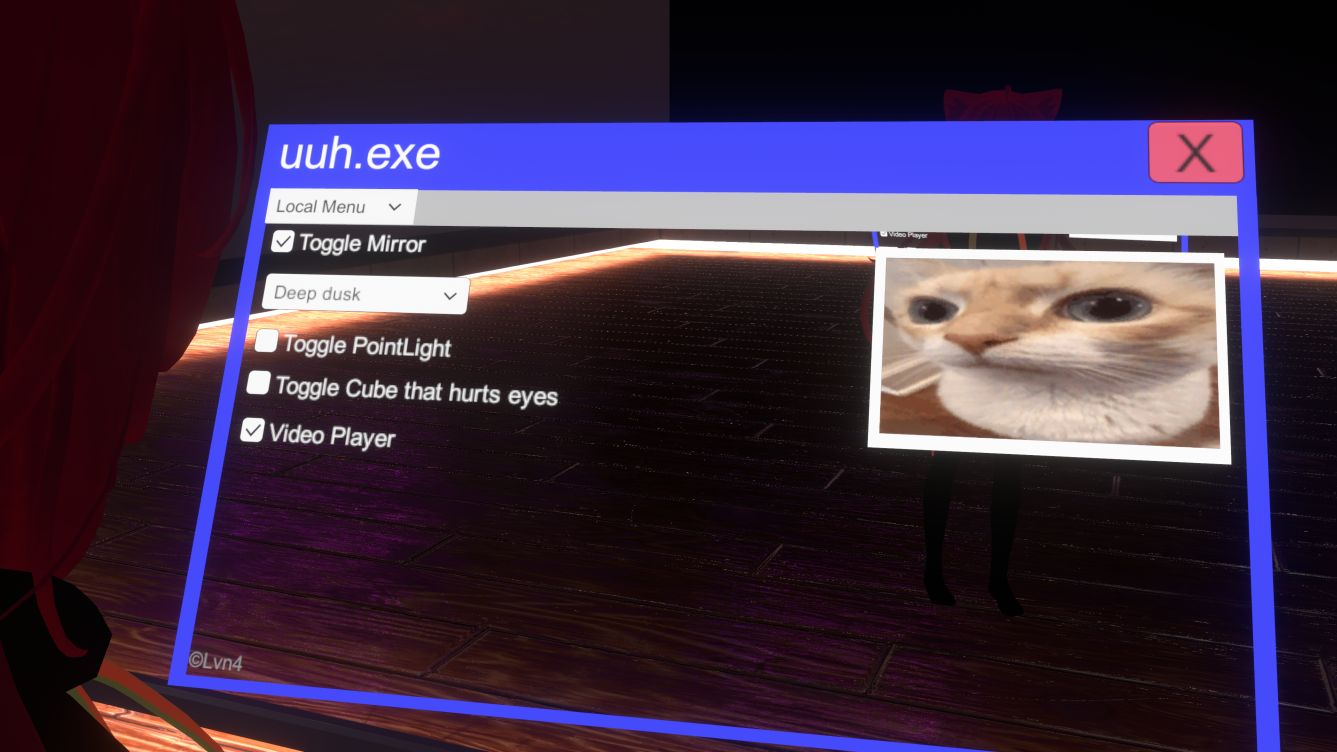
\includegraphics[width=1\textwidth]{pictures/Piotr/VRC_UI1.jpg}
    \caption{Very simple example of user interface in VRChat}
    \label{fig:vrc1}
\end{figure}
\pagebreak

\subsection{Przykładowa tabela}
kreatywno-autystyczne użycie tabeli ( Patrz \ref{tab:example_table_} ) 
\begin{table}[!h]
\begin{tabular}{@{}lllll@{}}
\toprule
\multicolumn{1}{|l}{S}   & \multicolumn{1}{r}{Z}                         & A                     & L                                & O                     \\ \midrule
N                        & \multicolumn{1}{l|}{A}                        & \multicolumn{1}{l|}{} & T                                & A                     \\ \midrule
B                        & E                                             & \multicolumn{1}{r}{L} & \multicolumn{1}{l|}{A}           & \multicolumn{1}{l|}{} \\ \midrule
\multicolumn{1}{|l|}{:3} & \begin{tabular}[c]{@{}l@{}}C\\ S\end{tabular} & hA                    & \multicolumn{1}{l|}{\textbf{AO}} & O                     \\ \cmidrule(r){1-4}
\end{tabular}
\caption{Przykład bardzo chaotycznej tabeli}
\label{tab:example_table_}
\end{table}
\subsection{Lista nie numerowana}
\begin{itemize}
    \item 2 fish (<><)
    \item aquarium.
    \item Gas station.
\end{itemize}
\subsection{Lista numerowana}
\begin{enumerate}
    \item Pierwsze coś.
    \item Meow.
    \item \textbf{Fascynująca} i \textbf{zmieniająca} pogląd na świat informacja. \label{enu:wow}
\end{enumerate}


\subsection*{ Przykładowy teskt }
\begingroup
\raggedright 
Akapit 1: Losowy cytat "Des larmes et des saints".
Les yeux ne voient rien. Catherine Emmerich a raison de dire qu’elle voit
par le cœur ! Le cœur étant la vue des saints, comment ne verraient-ils pas
plus loin que nous ? L’œil a un champ réduit, il voit toujours de l’extérieur.
Mais le monde étant intérieur au cœur, l’introspection est l’unique méthode
pour accéder à la connaissance. Le champ visuel du cœur ? Le Monde, plus
Dieu, plus le néant. C’est-à-dire tout.

Akapit 2: Przykładowy teskt zawierający formatowanie i odnośniki).
W rysunku \ref{fig:vrc1} widzimy interfejs użytkownika umożliwiający przełączanie różnych obiektów w scenie (Unity to silnik VRChat'a więc jeśli chcemy dodać coś do gry używamy odpowiedniej wersji Unity i SDK). Ważne jest dodatnie tutaj także odwołania do tabeli \ref{tab:example_table_} i listy \ref{enu:wow} żeby wszystko się zgadzało.
\begingroup

\ref{enu:wow}